\documentclass[nonacm]{acmart}

%%
%% \BibTeX command to typeset BibTeX logo in the docs
\AtBeginDocument{%
  \providecommand\BibTeX{{%
    \normalfont B\kern-0.5em{\scshape i\kern-0.25em b}\kern-0.8em\TeX}}}

%%
%% These commands are for a JOURNAL article.
%% PLEASE IGNORE THEM!
\acmJournal{TOIT}
\acmVolume{37}
\acmNumber{4}
\acmArticle{111}
\acmMonth{8}

%%
%% end of the preamble, start of the body of the document source.
\usepackage{textcomp}
\usepackage{multirow}
\usepackage{array}
\usepackage{hyperref}
\usepackage{graphicx}
\usepackage{float}

\usepackage{tikz}
\usetikzlibrary{shapes.geometric, arrows.meta, positioning}

\tikzset{
    box/.style={
        rectangle, rounded corners=3pt,
        minimum width=2.4cm, minimum height=0.9cm,
        text centered, draw=black, fill=gray!10,
        font=\small
    },
    decision/.style={
        diamond, aspect=2,
        minimum width=2.8cm, minimum height=0.9cm,
        text centered, draw=black, fill=gray!10,
        font=\small
    },
    arrow/.style={-{Stealth[length=5pt]}, thick}
}


\newcolumntype{M}[1]{>{\centering\arraybackslash}m{#1}}
\newcommand{\bla}{blah blah blah blah blah blah blah blah blah blah blah blah blah blah blah blah}
%Definition of Colors - Start
\definecolor{xred}{RGB}{255,0,0}
\definecolor{xblue}{RGB}{68,114,196}
\definecolor{xgreen}{RGB}{0,176,80}
\definecolor{xpurple}{RGB}{112,48,160}
\definecolor{xorange}{RGB}{237,125,49}
%Definition of Colors - End

\setcopyright{none}
\settopmatter{printacmref=false} % Removes citation information below abstract
\renewcommand\footnotetextcopyrightpermission[1]{} % removes footnote with conference information in first column
\pagestyle{plain}
\begin{document}

\title{The Cost of Zero-Trust for Smart-Lock Systems}

\author{Christophe-Mokili Andunda (\lowercase{2210781001@fh-burgenland.at})}

\author{Benjamin Huang Weixiang (\lowercase{2210781004@fh-burgenland.at})}

\begin{abstract}
\textbf{ABSTRACT:}
Digitalization has increasingly transformed physical infrastructures into connected cyber-physical systems (CPS). Buildings, shared facilities, rental spaces, and workplaces are no longer managed only through manual processes, but through software platforms, cloud services, Application Programming Interfaces (APIs), and connected devices. In this context, digital access control has become especially relevant, because decisions about physical entry are increasingly handled by cloud-based systems.

Simple mechanisms such as static keypad codes are easy to deploy and use, but they can be shared, leaked, or reused indefinitely without any check at the moment of entry. Stronger access control mechanisms address this by re-verifying a request at the moment of access. This leads to a security-cost trade-off: higher assurance can reduce the risk of unauthorized access, but it also increases infrastructure resource usage, operational complexity, and cloud cost.

This paper examines this trade-off using a microservice-based booking platform for music studios deployed on Amazon Web Services (AWS). The system consists of a User Service, Studio Service, Booking Service, and Access Service. Three access control scenarios with increasing security levels are implemented and compared. The first scenario generates the access code at booking time, and the code is then valid on its own with no further check at the door. The second scenario instead generates the code only at the door, after the system validates the booking code against the current time window. The third scenario builds upon the second by additionally requiring a face verification step before the code is generated, confirming that the person present at the door matches the booking.

To quantify this trade-off, the evaluation measures cost per access attempt, average Central Processing Unit (CPU) utilization, and average memory utilization. These metrics are selected because they show how additional verification logic affects the infrastructure footprint of the Access Service, which contains the scenario-specific access control logic. By comparing the three scenarios under the same deployment conditions, this work provides a practical basis for analyzing the operational cost of stronger access control in smart-lock-based CPS.
\end{abstract}

\maketitle

\newpage
\section{Introduction}

Cyber-Physical Systems (CPS) and the so-called Internet of Things (IoT)-based access control solutions are increasingly relevant in domains such as smart homes, short-term rentals, shared facilities, and building automation. In particular, smart locks enable flexible, cloud-based management of access permissions and support automated processes such as check-in and check-out. These systems consist of multiple interacting components, including user interfaces, cloud services, databases, Application Programming Interfaces (APIs), and physical devices.

The adoption of smart locks has grown rapidly in recent years, with the global market expected to reach over US\$8 billion by 2030 \cite{refMarket}. Platforms such as Airbnb rely on smart locks to enable automated check-in and remote access management, eliminating the need for physical key exchange. As a result, access control is no longer purely physical but is increasingly mediated through software systems, APIs, and cloud services. This increases system complexity and introduces additional attack surfaces.

This increase in potential attack surfaces is accompanied by growing security concerns. Prior research has shown that Bluetooth-based smart locks can be vulnerable to eavesdropping and man-in-the-middle attacks \cite{refBluetooth}, while replay attacks can enable unauthorized unlocking by reusing captured communication \cite{diao2025masterlock}. Additionally, flaws in smart home platforms have shown that attackers can inject credentials or unlock doors via compromised cloud services \cite{refSmartHome}. These findings highlight that smart lock systems can introduce vulnerabilities across device, communication, and cloud layers.

This leads to a fundamental trade-off between usability, security, and infrastructure cost. Simple mechanisms such as static keypad codes are easy to use, but they are vulnerable to sharing, leakage, and unauthorized reuse. In contrast, stronger access control mechanisms, such as contextual validation or biometric verification, can improve protection but may also increase operational cost, Central Processing Unit (CPU) usage, memory usage, and system complexity. Similar to prior work on the measurable cost of security mechanisms, such as the cost introduced by the Hypertext Transfer Protocol Secure (HTTPS) \cite{naylor2014cost}, enhanced access control in smart-lock-based systems can also create measurable infrastructure overhead.

In this position paper, we investigate this trade-off in the context of bcube, a cloud-based booking platform for music studios. The system follows a microservice architecture and consists of a User Service, Studio Service, Booking Service, and Access Service. A Nuki Smart Lock is used as the physical access mechanism, while the cloud-based Access Service controls when a valid access code is generated or released.

We compare three access control scenarios with increasing security levels. The first scenario uses direct keypad access after a completed booking. The second scenario requires booking-code validation before a temporary keypad access code is generated. The third scenario additionally includes face verification before the access code is generated. The goal is to evaluate how these different security levels affect operational cost and infrastructure resource usage.

The evaluation focuses on three concrete metrics: cost per access attempt, average CPU utilization, and average memory utilization. These metrics are measured mainly for the Access Service, because it contains the scenario-specific access logic and is expected to show the clearest differences between the implemented security levels.

The remainder of this paper is structured as follows: Section II reviews related work, Section III presents the methodology and experimental setup, and Section IV concludes the paper.
\newpage
\section{Related Work}

The cost of security mechanisms has been widely studied, particularly in the context of network protocols. 
A key reference is \cite{naylor2014cost}, where the authors evaluated the cost of the "S" in HTTPS, demonstrating that adding security through TLS introduces additional data overhead and computational cost. This work provides a foundation for analyzing security not only as a functional property, but also as a measurable source of resource consumption.

In the context of Cyber-Physical Systems (CPS), Ivki\'c et al. \cite{ref01, ref02, ref03} propose a series of security cost modeling frameworks that highlight the importance of evaluating security mechanisms alongside their resource and operational overhead. First, Ivki\'c et al. \cite{ref01} introduced the concept of modeling security costs in terms of resource consumption, showing that such mechanisms can significantly affect constrained environments. Next, they extended this by proposing a runtime framework \cite{ref02}, demonstrating that security overhead varies dynamically with system state and workload. Finally, they presented a more comprehensive model integrating computational, communication, and operational costs \cite{ref03}, emphasizing the need for holistic evaluation of security decisions.

Recent work has identified security vulnerabilities in smart lock systems across several components. Ho et al. \cite{ho2016smartlocks} analyze five commercial smart locks and show that weaknesses can arise not only from implementation bugs, but also from system design, revocation handling, access logging, and automatic unlocking interaction models. Caballero-Gil et al. \cite{caballero2023smartlocks} and Turk \cite{turk2023smartlock} report weaknesses in Bluetooth communication, including replay and interception attacks, while Diao et al. \cite{diao2025masterlock} identify vulnerabilities in device protocols that allow unauthorized access persistence and manipulation of access rights. Veijalainen and Karlsson \cite{veijalainen2021evaluating} complement these works with a threat-model-driven penetration test of a smart door lock system, deriving concrete tests from reconnaissance and STRIDE/DREAD-based threat modeling to analyze app-server communication, replay behavior, gateway exposure, and key-tag access. Together, these works show that vulnerabilities in smart lock systems can already arise at the device and communication layer, before any cloud-side access control logic is even involved.

Beyond the device and communication layer, vulnerabilities have also been identified in the companion mobile applications that control smart locks. Allen et al. \cite{allen2024androidiot} highlight security flaws in companion mobile applications, such as exposure of API endpoints and authentication mechanisms. Complementing these findings, Wang et al. \cite{wang2019mirror} propose a scalable methodology to detect such issues through the analysis of mobile companion applications, showing that insecure design patterns can propagate across multiple devices due to code reuse. Together with the device-level findings above, these results demonstrate that vulnerabilities can occur at different layers of smart lock systems, motivating the need for stronger access control mechanisms.

User-oriented research further shows that smart lock security cannot be evaluated only from a technical perspective. Hazazi and Shehab \cite{hazazi2024automation} investigate smart lock automation in smart home environments and show that users perceive such automation in terms of security, convenience, awareness, privacy, and reliability. This is relevant for access-control systems because stronger verification mechanisms must not only improve protection, but also remain understandable and acceptable for users.

% Recent work has identified security vulnerabilities in smart lock systems across several components. Caballero-Gil et al. \cite{caballero2023smartlocks} and Turk \cite{turk2023smartlock} report weaknesses in Bluetooth communication, including replay and interception attacks, while Diao et al. \cite{diao2025masterlock} identify vulnerabilities in device protocols that allow unauthorized access persistence and manipulation of access rights. In addition, Allen et al. \cite{allen2024androidiot} highlight security flaws in companion mobile applications, such as exposure of API endpoints and authentication mechanisms. Complementing these findings, Wang et al. \cite{wang2019mirror} propose a scalable methodology to detect such issues through the analysis of mobile companion applications, showing that insecure design patterns can propagate across multiple devices due to code reuse. Together, these works demonstrate that vulnerabilities can occur at different layers of smart lock systems, motivating the need for stronger access control mechanisms.

Two complementary implementation-oriented studies investigate the integration of smart lock systems with cloud infrastructures. Salvadore \cite{salvadore2022smartlocks} proposes a cloud-based orchestration system built on API-based integration with smart lock platforms such as Nuki, where the Web API is used to generate and manage time-limited virtual keys based on booking data. This enables automated access provisioning and reduces manual intervention. However, this approach relies mainly on booking data and does not evaluate additional verification at access time.

In contrast, Zebic \cite{zebic2023azure} examines the integration of a Nuki smart lock into Microsoft Azure from a process-oriented perspective. The work identifies and evaluates the individual steps required for integration, such as configuring authentication parameters, establishing API connections, and managing device-specific settings. By introducing metrics to assess the complexity of these steps, the study shows that integrating smart locks into cloud environments involves multiple configuration tasks that go beyond simple API usage.

Other prototype-based studies illustrate how smart locks can be implemented using embedded devices and cloud services. Maurya et al. \cite{maurya2020cloudnative} implement a cloud-native door lock system using Raspberry Pi, Arduino, Alexa, and Amazon Web Services, including services for image storage, face recognition, messaging, and device communication. Derbali \cite{derbali2023iotsdl} proposes an Internet of Things smart door lock system with temporary PIN codes, Radio Frequency Identification, Bluetooth-based access, remote unlocking, and access records. Zheng et al. \cite{zheng2024stm32} present an STM32-based smart door lock with multiple unlocking methods, including RFID, fingerprint recognition, keypad access, remote unlocking, and a vibration alarm. These works demonstrate the technical feasibility of cloud-connected and embedded smart lock systems.

While existing work has extensively analyzed security vulnerabilities, usability concerns, and system integration challenges in smart lock environments, the infrastructure cost associated with stronger access control mechanisms has not been studied as extensively. Additional verification steps, such as contextual validation or biometric verification, can improve access control but also introduce more complex system interactions, additional cloud service usage, and increased resource consumption.

To address this gap, this position paper focuses on the cost and infrastructure impact of stronger access control mechanisms in a cloud-managed smart lock system. By comparing three access control scenarios with increasing security levels, ranging from direct keypad access to booking-code validation and face verification, this work evaluates how stronger access control affects operational cost, CPU utilization, and memory utilization in a realistic cloud-based booking system.
\newpage
\section{Methodology}

This chapter describes the methodological design used to evaluate the cost of stronger access control in a smart-lock-based booking system. The evaluation follows a comparative approach: the same booking and access use case is implemented with three different access control scenarios, each representing a different security level. The scenarios are then compared using cloud cost and infrastructure resource metrics.

\subsection{High-Level Use Case}

The use case considered in this work is a booking-based access control process for music studios. A user books a studio for a specific time window and should only be able to enter the room during this valid booking period. The physical entry point is protected by a Nuki Smart Lock and keypad, while the access decision is controlled by a cloud-based backend system.

At a high level, the process consists of four steps. First, a user creates a booking for a studio. Second, the system stores the booking and associates it with a valid access period. Third, the user attempts to access the studio at the door. Fourth, the system either grants or denies access depending on the selected access control scenario. This is illustrated in Figure~\ref{fig:high_level_use_case}.

This leads to a security-cost trade-off: higher assurance can reduce the risk of unauthorized access, but it also increases infrastructure resource usage, operational complexity, and cloud cost.

\begin{figure}[H]
\centering
\resizebox{\linewidth}{!}{%
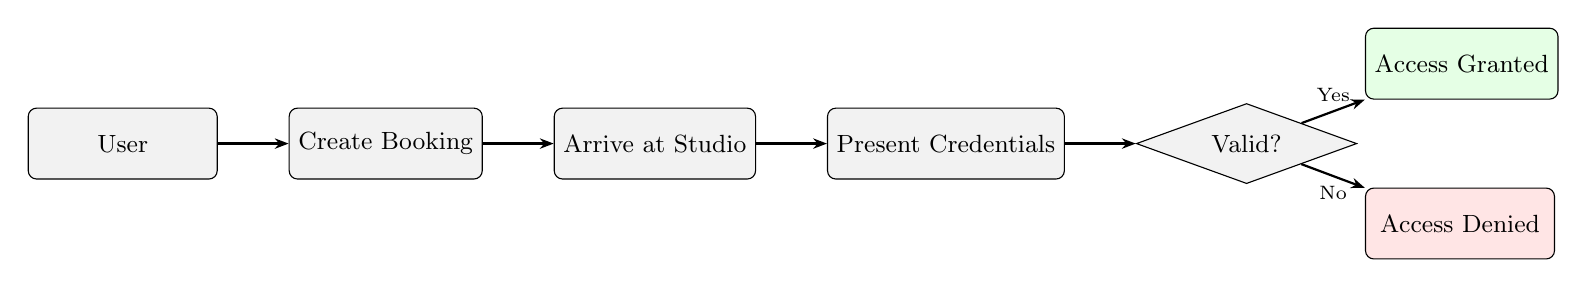
\begin{tikzpicture}[node distance=0.5cm and 0.9cm]

    \node[box] (user)    {User};
    \node[box, right=of user]    (book)    {Create Booking};
    \node[box, right=of book]    (arrive)  {Arrive at Studio};
    \node[box, right=of arrive]  (verify)  {Present Credentials};
    \node[decision, right=of verify] (check) {Valid?};
    \node[box, above right=0.3cm and 0.8cm of check, fill=green!10] (grant) {Access Granted};
    \node[box, below right=0.3cm and 0.8cm of check, fill=red!10]   (deny)  {Access Denied};

    \draw[arrow] (user)   -- (book);
    \draw[arrow] (book)   -- (arrive);
    \draw[arrow] (arrive) -- (verify);
    \draw[arrow] (verify) -- (check);
    \draw[arrow] (check)  -- node[above, font=\scriptsize]{Yes} (grant);
    \draw[arrow] (check)  -- node[below, font=\scriptsize]{No}  (deny);

\end{tikzpicture}%
}
\caption{High-level booking and access control use case.}
\label{fig:high_level_use_case}
\end{figure}

\subsection{System Architecture and Roles}

The prototype is implemented as a microservice application consisting of four Spring Boot 3.5.6 services deployed on AWS ECS Fargate and exposed via an Application Load Balancer (ALB) with path-based routing rules. All services persist data in dedicated Amazon RDS PostgreSQL 17 databases on a \texttt{db.t3.micro} instance. Table~\ref{tab:responsibilities} summarizes the main roles of the system components.

\begin{table}[H]
\centering
\caption{System roles and responsibilities}
\label{tab:responsibilities}
\begin{tabular}{p{1.2cm}p{3.2cm}p{8.0cm}}
\hline
\textbf{ID} & \textbf{Component} & \textbf{Responsibility} \\
\hline
R1 & User Service      & Manages authentication and user data. Issues JWT tokens signed with a shared HMAC-SHA256 secret and validates incoming Bearer tokens using Spring Security's JWT decoder. \\
R2 & Studio Service    & Manages studio entities, availability, and Nuki smartlock associations. \\
R3 & Booking Service   & Creates and stores bookings, including the booked studio, user, and valid time window. Upon booking creation, it synchronously calls the Access Service to initialize the access permission. \\
R4 & Access Service    & Implements the scenario-specific access control logic. This is the primary measurement subject in this evaluation. \\
R5 & Nuki Smart Lock   & Provides the physical access mechanism. The lock executes time-limited keypad codes registered by the Access Service via the Nuki Web API. \\
\hline
\end{tabular}
\end{table}

The Access Service (R4) is deployed as a single ECS Fargate task with 0.25 vCPU and 512\,MB memory. The active security scenario is selected at startup via the \texttt{FA\_LEVEL} environment variable, which activates the corresponding implementation through Spring Boot's \texttt{@ConditionalOnProperty} mechanism. All three implementations share a common abstract base class and differ only in the access-time flow.

For face verification (Cases 2 and 3), the system relies on a pre-built Amazon Rekognition face collection. User face enrollment is handled by a separate service in a distinct repository, implementing the following pipeline: a user photo is uploaded to Amazon S3, which triggers an AWS Lambda function that invokes the Rekognition \texttt{IndexFaces} API and stores the resulting \texttt{FaceId} and user identity in Amazon DynamoDB. This enrollment pipeline runs once per user and is independent of the per-access-attempt flow evaluated in this work.

\subsection{Access Control Scenarios}

Three access control scenarios are implemented and compared. They represent increasing security levels and differ in how much verification is performed at the moment of access.

\textbf{Case 1: Single-Factor Access (1FA).}
At booking creation, the Access Service generates a six-digit PIN, encrypts and stores it in PostgreSQL, and immediately registers a time-limited keypad code on the Nuki lock via the Nuki Web API. At access time, the user enters this PIN directly at the Nuki keypad without any further backend interaction. The sole authentication factor is knowledge of the booking code. No AWS managed services are invoked per access attempt.

\textbf{Case 2: Two-Factor Access (2FA).}
At booking creation, the Access Service stores the encrypted PIN in the database without registering a Nuki code. At access time, the following steps are performed: (1) the user submits the booking PIN on a separate dashboard, which the Access Service validates against a stored SHA-256 hash. (2) The user captures a selfie, which the Access Service passes in-memory to the Amazon Rekognition API against the pre-built face collection. (3) Upon successful biometric verification, the Access Service generates a new Nuki code, registers it via the Nuki Web API, and returns it to the application for display. The two authentication factors are knowledge of the booking code and biometric identity.

\textbf{Case 3: Three-Factor Access (3FA).}
Case 3 is identical to Case 2 in all steps except the delivery of the Nuki code. Instead of returning the code to the application for display, the Access Service invokes Amazon SES to send the code to the user's registered email address. The code is not shown in the application. The three authentication factors are knowledge of the booking code, biometric identity, and possession of the registered email account.

\begin{figure}[H]
\centering
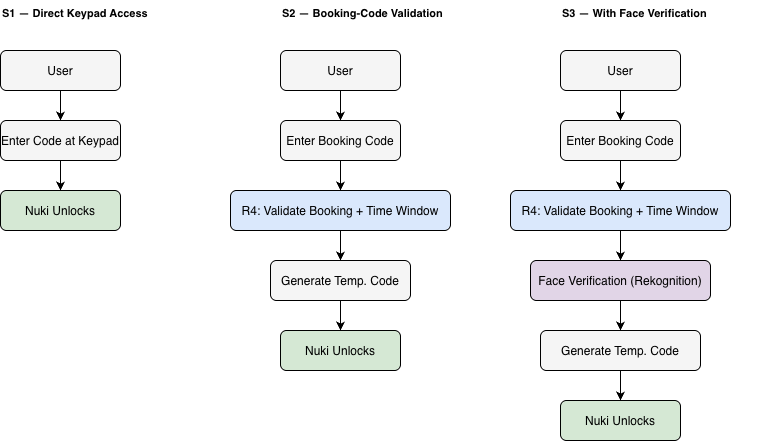
\includegraphics[width=\linewidth]{fig/scenarios.png}
\caption{Comparison of the three access control scenarios with mapped evaluation metrics.}
\label{fig:scenario_comparison}
\end{figure}

\subsection{Evaluation Metrics}

The evaluation uses three metrics to quantify the cost of stronger access control. The metrics focus on the Access Service because it contains the scenario-specific access logic. The User Service, Studio Service, and Booking Service behave identically across all scenarios and are excluded from metric collection accordingly.

\begin{itemize}
    \item \textbf{M1: Cost per Access Attempt.}
    The average variable AWS service cost per access attempt in each scenario. Calculated by dividing the total scenario-related variable cloud cost by the number of executed access attempts. Fixed infrastructure costs (ECS Fargate, RDS, VPC, ALB) are excluded as they are invariant across scenarios.

    \item \textbf{M2: Average CPU Utilization.}
    The average CPU utilization of the Access Service during the test window, reported as a percentage of the allocated 0.25 vCPU, collected via Amazon CloudWatch Container Insights at one-minute granularity.

    \item \textbf{M3: Average Memory Utilization.}
    The average memory utilization of the Access Service during the test window, reported as a percentage of the allocated 512\,MB, collected via Amazon CloudWatch Container Insights at one-minute granularity.
\end{itemize}

The cost per access attempt (M1) is calculated as follows:

\begin{equation}
\text{M1} = \frac{\text{Total Scenario-Related Variable AWS Cost}}{\text{Number of Access Attempts}}
\end{equation}

\subsection{Measurement and Data Collection}

Variable cost data is derived from AWS public pricing as of June 2026, applied to the exact number of external service invocations per access attempt. At access time, Case 2 invokes one Rekognition \texttt{SearchFacesByImage} call (\$0.001 per image). Case 3 additionally invokes one Amazon SES send (\$0.0001 per message). Case 1 invokes no AWS managed services at access time. The face enrollment pipeline (S3, Lambda, \texttt{IndexFaces}, DynamoDB) is a one-time per-user operation and is excluded from per-attempt cost calculations. The Nuki Web API is billed externally to AWS and is also excluded.

Fixed infrastructure costs (ECS Fargate, RDS, VPC, ALB) are treated as a shared baseline invariant across all three scenarios and are reported separately for reference.

CPU and memory utilization metrics are collected via Amazon CloudWatch Container Insights for the Access Service ECS task, using one-minute average statistics. Because all three scenarios run on identical task configurations (0.25 vCPU, 512\,MB), the reported percentages are directly comparable without normalization.

\subsection{Test Execution}

Each scenario is executed under identical infrastructure conditions. The same ECS task configuration, RDS instance class, ALB listener rules, and CloudWatch monitoring setup are applied consistently. No auto-scaling policies are active during the test window.

For each scenario, 20 bookings and 20 corresponding access attempts are executed sequentially via the application under controlled conditions. All three runs are conducted on 2026-06-18 with the \texttt{FA\_LEVEL} environment variable set to \texttt{1}, \texttt{2}, and \texttt{3} for Case 1, Case 2, and Case 3, followed by an ECS force redeployment between scenarios.

After execution, data is grouped by scenario and evaluated against M1, M2, and M3.

\newpage
\section{Results and Analysis}

\subsection{Overview of Results}

This section presents the measured results for all three access control scenarios across the three evaluation metrics: cost per access attempt (M1), average CPU utilization (M2), and average memory utilization (M3). All scenarios were executed with 20 bookings and 20 corresponding access attempts under identical infrastructure conditions.

Table~\ref{tab:results_overview} provides a summary of all measured values. Cost figures include the fixed monthly infrastructure baseline of \$4.43 amortized over 1{,}000 access attempts, making the comparison practically meaningful.

\begin{table}[H]
\centering
\caption{Measured results per scenario (cost at 1{,}000 monthly access attempts)}
\label{tab:results_overview}
\begin{tabular}{p{1.5cm}p{2.2cm}p{3.2cm}p{2.6cm}p{2.6cm}}
\hline
\textbf{Case} & \textbf{Security Level} & \textbf{M1 (Total/Month)} & \textbf{M2 (Avg. CPU)} & \textbf{M3 (Avg. Mem.)} \\
\hline
Case 1 & Low    & \$4.43 & 3.1\% & 41.2\% \\
Case 2 & Medium & \$5.43 & 3.4\% & 41.8\% \\
Case 3 & High   & \$5.53 & 3.3\% & 42.1\% \\
\hline
\end{tabular}
\end{table}

\subsection{Cost per Access Attempt (M1)}

The total monthly cost of operating the system consists of two components: a fixed infrastructure baseline that is invariant across all scenarios, and a variable per-attempt cost that depends on the managed AWS services invoked during each access event.

\paragraph{Fixed Infrastructure Baseline.}
The shared ECS Fargate task, RDS \texttt{db.t3.micro} instance, VPC, and ALB components incur a combined fixed cost of \$4.43 per month regardless of which access control scenario is active or how many access attempts are processed. This baseline represents the minimum operational cost of running the system and is identical for all three cases.

\paragraph{Variable Cost per Attempt.}
Case 1 invokes no external AWS services at access time and therefore adds no variable cost on top of the baseline. Case 2 introduces a single call to Amazon Rekognition \texttt{SearchFacesByImage} per access attempt, priced at \$0.001 per image (AWS pricing, June 2026). Case 3 is identical to Case 2 but additionally dispatches the Nuki code via Amazon SES, priced at \$0.0001 per message, bringing its per-attempt variable cost to \$0.0011.

Table~\ref{tab:cost_breakdown} breaks down the variable cost components per scenario.

\begin{table}[H]
\centering
\caption{Variable cost breakdown per access attempt (AWS pricing, June 2026)}
\label{tab:cost_breakdown}
\begin{tabular}{p{1.5cm}p{3.5cm}p{2.8cm}p{2.8cm}}
\hline
\textbf{Case} & \textbf{Service Invocation} & \textbf{Unit Price (USD)} & \textbf{Variable Total} \\
\hline
Case 1 & None & -- & \$0.0000 \\
\hline
Case 2 & Rekognition \texttt{SearchFacesByImage} & \$0.0010 & \$0.0010 \\
\hline
\multirow{2}{*}{Case 3} & Rekognition \texttt{SearchFacesByImage} & \$0.0010 & \multirow{2}{*}{\$0.0011} \\
                         & Amazon SES (1 message)                  & \$0.0001 & \\
\hline
\end{tabular}
\end{table}

\paragraph{Total Monthly Cost.}
Table~\ref{tab:monthly_cost} combines the fixed baseline with the projected variable cost at three usage volumes to illustrate how the cost structure shifts with scale.

\begin{table}[H]
\centering
\caption{Total projected monthly cost including fixed infrastructure baseline}
\label{tab:monthly_cost}
\begin{tabular}{p{1.5cm}p{2.0cm}p{2.2cm}p{2.2cm}p{2.2cm}}
\hline
\textbf{Case} & \textbf{Fixed} & \textbf{100 att.} & \textbf{1{,}000 att.} & \textbf{10{,}000 att.} \\
\hline
Case 1 & \$4.43 & \$4.43 & \$4.43  & \$4.43  \\
Case 2 & \$4.43 & \$4.53 & \$5.43  & \$14.43 \\
Case 3 & \$4.43 & \$4.54 & \$5.53  & \$15.43 \\
\hline
\end{tabular}
\end{table}

At low usage (100 attempts/month), the fixed baseline dominates and all three scenarios cost nearly the same (\$4.43 to \$4.54). At 1{,}000 attempts the security surcharge of Case 3 over Case 1 is \$1.10 (+24.8\%). At 10{,}000 attempts the variable cost of Case 3 (\$11.00) exceeds the fixed infrastructure cost by a factor of approximately 2.5, making the choice of security scenario the primary cost driver.

\subsection{CPU and Memory Utilization (M2, M3)}

Both CPU and memory utilization of the Access Service remained at comparable levels across all three scenarios, as shown in Table~\ref{tab:results_overview}. The observed variation (3.1\% to 3.4\% for CPU, 41.2\% to 42.1\% for memory) falls within the margin of measurement noise inherent to one-minute CloudWatch sampling and does not represent a meaningful operational difference.

This outcome is consistent with the architectural design of the system. The Access Service is I/O-bound: its main role at access time is to invoke external managed services (Rekognition, SES) and await their responses. The computationally intensive operations, namely face recognition inference and email relay, are executed on AWS-managed infrastructure and do not contribute to the Access Service's CPU or memory footprint. The additional Rekognition and SES calls introduced by Cases 2 and 3 manifest as network round-trips and API latency, not as additional local compute load.

The memory footprint of approximately 41 to 42\% across all scenarios corresponds to the baseline JVM heap usage of the Spring Boot application and the in-memory image buffer used during face verification. Since the selfie image is passed directly to the Rekognition API and not persisted, its transient allocation does not accumulate over repeated attempts.

Consequently, M2 and M3 are not suitable discriminating metrics for the scenarios evaluated in this work. The relevant resource impact of higher security levels is captured entirely by M1.

\subsection{Comparison of Security Levels}

Figure~\ref{fig:cost_comparison} illustrates the total monthly cost at 1{,}000 access attempts across the three scenarios, combining the fixed baseline with scenario-specific variable costs. The step from Case 1 to Case 2 represents the dominant cost increment, driven entirely by the Rekognition integration. The additional surcharge from Case 2 to Case 3 (SES delivery) is marginal in comparison.

\begin{figure}[H]
\centering
\resizebox{0.78\linewidth}{!}{%
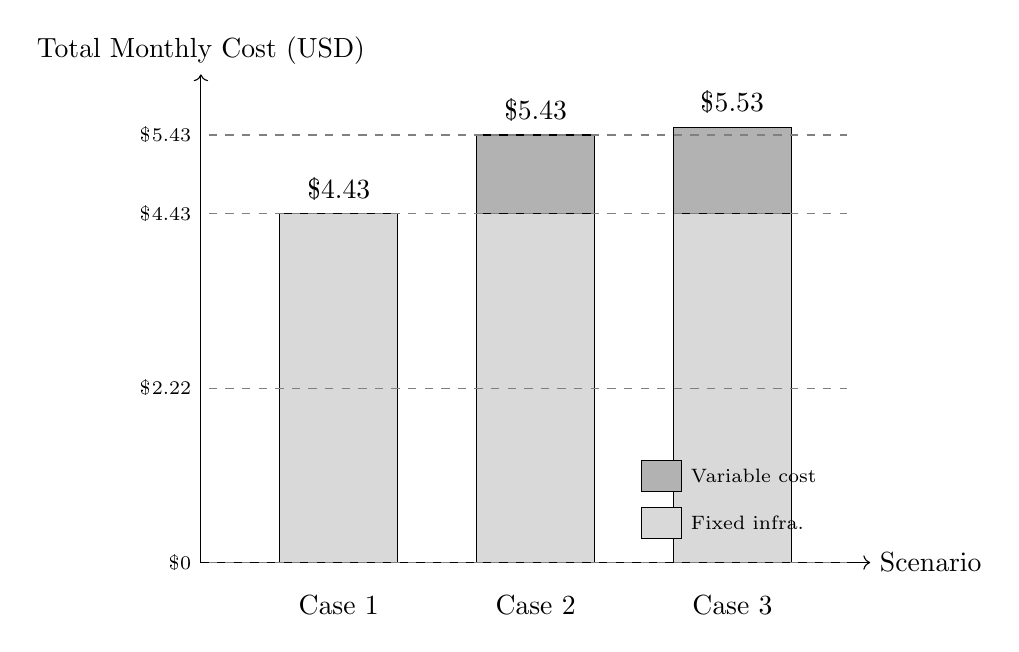
\begin{tikzpicture}
    \draw[->] (0,0) -- (8.5,0) node[right] {Scenario};
    \draw[->] (0,0) -- (0,6.2) node[above] {Total Monthly Cost (USD)};

    % Fixed baseline layer (gray)
    \draw[fill=gray!30] (1,0)   rectangle (2.5,4.43);
    \draw[fill=gray!30] (3.5,0) rectangle (5.0,4.43);
    \draw[fill=gray!30] (6.0,0) rectangle (7.5,4.43);

    % Variable cost layer (darker)
    \draw[fill=gray!60] (3.5,4.43) rectangle (5.0,5.43);
    \draw[fill=gray!60] (6.0,4.43) rectangle (7.5,5.53);

    \node[below] at (1.75,-0.3) {Case 1};
    \node[below] at (4.25,-0.3) {Case 2};
    \node[below] at (6.75,-0.3) {Case 3};

    \node[above] at (1.75,4.48) {\$4.43};
    \node[above] at (4.25,5.48) {\$5.43};
    \node[above] at (6.75,5.58) {\$5.53};

    \foreach \y/\label in {0/\$0, 2.215/\$2.22, 4.43/\$4.43, 5.43/\$5.43} {
        \draw[gray, dashed] (0.1,\y) -- (8.2,\y);
        \node[left, font=\scriptsize] at (0,\y) {\label};
    }

    % Legend
    \draw[fill=gray!30] (5.6,0.3) rectangle (6.1,0.7);
    \node[right, font=\scriptsize] at (6.1,0.5) {Fixed infra.};
    \draw[fill=gray!60] (5.6,0.9) rectangle (6.1,1.3);
    \node[right, font=\scriptsize] at (6.1,1.1) {Variable cost};
\end{tikzpicture}%
}
\caption{Total monthly cost by scenario at 1{,}000 access attempts (fixed + variable).}
\label{fig:cost_comparison}
\end{figure}

\subsection{Interpretation of Findings}

The results confirm that the fixed infrastructure baseline (\$4.43/month) is the dominant cost component at low to moderate access volumes. At 1{,}000 monthly attempts, it accounts for 80\% of the total cost in Case 3. The choice of security scenario therefore has limited practical cost impact until access volumes reach several thousand attempts per month.

When variable costs become significant at higher volumes, the primary driver is the integration of Amazon Rekognition for biometric face verification (Case 2 and 3), not the out-of-band delivery channel (Case 3 only). Rekognition accounts for \$0.001 of the \$0.0011 per-attempt cost in Case 3, approximately 91\% of the total variable cost of the highest-security scenario. The SES surcharge of \$0.0001 per attempt is negligible by comparison.

The absence of measurable differences in CPU and memory utilization across scenarios reflects the delegation model inherent to cloud-native architectures: managed services externalize computational work, making on-task resource metrics an unreliable proxy for security-related operational cost. The true cost of higher security assurance is best captured through API billing metrics rather than infrastructure utilization metrics.

\newpage
\section{Limitations and Future Work}

The scenario design in this work is informed by the common distinction between authentication factors — something the user \textit{knows}, something the user \textit{has}, and something the user \textit{is} — as defined in NIST SP 800-63B~\cite{nist80063b}. However, the three scenarios do not constitute single-, two-, and three-factor authentication in the formal sense of this standard. NIST SP 800-63B defines possession-based factors as physical or cryptographic authenticators, such as hardware tokens or cryptographic keys bound to a device. A booking code does not meet this definition because it is a knowledge-based secret that can be copied, shared, or forwarded. S2 therefore does not introduce a second authentication factor; instead, its security gain comes from contextual enforcement at the moment of entry rather than from a distinct possession factor.

A second limitation concerns the scale of the evaluation. Each scenario was executed with 20 bookings and 20 access attempts under controlled and identical infrastructure conditions. While this allows for a direct comparison between scenarios, it does not reflect production-scale traffic patterns, concurrent access attempts, or variable load conditions. The observed cost and resource usage values should therefore be interpreted as indicative rather than representative of real-world deployments.

Finally, the evaluation focuses exclusively on the Access Service (R4) as the measurement point. Costs and resource usage associated with supporting services such as Amazon Rekognition, the Nuki Web API, or the database layer are included in the cost metric M1 but are not individually isolated. This means that the contribution of each external dependency to the overall cost difference between scenarios cannot be precisely attributed from the current measurements alone.
\newpage
\section{Conclusion}

Access control in IoT-enabled physical spaces sits at the intersection of security engineering and cloud economics. As smart lock systems move from simple PIN-based mechanisms to biometric and multi-factor verification, the cost implications of that transition remain underexplored in practice.

This work addresses the question of how much stronger access control actually costs in a deployed cloud environment. The gap between theoretical security gains and their operational price is rarely quantified in concrete, reproducible terms.

To answer this, a prototype booking and access system was implemented as four Spring Boot microservices on AWS ECS Fargate and evaluated across three scenarios: single-factor PIN access (1FA), two-factor biometric verification via Amazon Rekognition (2FA), and three-factor verification with out-of-band code delivery via Amazon SES (3FA).

The central finding is that the cost of stronger access control is dominated by the integration of managed AI inference services, not by compute or infrastructure overhead. Moving from 1FA to 3FA adds \$0.0011 per access attempt in variable costs, with Rekognition accounting for 91\% of that figure. CPU and memory utilization of the Access Service remain indistinguishable across all three scenarios, as the computationally intensive work is offloaded to AWS-managed infrastructure. At moderate usage volumes, the fixed infrastructure baseline of \$4.43 per month outweighs the security surcharge by a wide margin.

Future work should investigate the cost behavior at higher access volumes, evaluate caching strategies to reduce repeated Rekognition invocations for frequent users, and extend the comparison to additional physical access scenarios beyond music studio bookings.

\newpage
\input{section/references}

\end{document}
\endinput
%%
%% End of file `sample-acmlarge.tex'.
